\section{Implementation}

\subsection{About Ngene}
\emph{Ngene} is a flexible, generic, multi-purpose genetic algorithm engine written in C++ with heavy emphasis on performance and flexibility. The engine is divided into logical modules that can be interchanged or extended upon in order to fit the intended goal.

The engine started out as an assignment for a sub-symbolic artificial intelligence course. It was written in Python, and 

\subsubsection{Modular Design}
The design is broken into the following modules:

\begin{itemize}
	\item (core) - The genetic algorithm itself
	\item Fitness - Assesses the fitness of a genotype
	\item Genotype - Produces the genotype and translates them to phenotype
	\item Mating - Crosses two genotypes
	\item Mutator - Mutates a genotype
	\item Selector - Selects a random genotype
\end{itemize}

All modules are loaded into memory when the program is executed and kept there until the program is terminated. This modular design is essential when it comes to making the engine available for all purposes. For example, while \emph{tournament} selection is suitable for most of the experiments in this thesis, other users may want to run a comparison test between different selection methods. This is easily achieved by simply specifying which module to use in a configuration file. There is no need to recompile a single line of code unless a new module is required. This modular design also keeps the code cleaner and easier to maintain.

\subsection{Why C++?}
Choosing a programming language depends on what kind of programme you want to write. A simple program with no special requirements can be written in any language. However performance becomes essential, there are really only two ways to code: In assembly (or machine code) or C/C++. Unlike languages that depend on a virtual machine (C\#, Java), or an interpreter (Common LISP, Python), code written in C/C++ is compiled directly to machine code before executed, usually yielding a much better performance.

Being a middle level language, C++ has many disadvantages when compared to today's higher level programming languages. For instance, all memory management must be explicitly handled in the code because C++ lacks a garbage collection found typically in C\# or Java. This means that we have to be careful of memory leaks and accessing valid memory addresses. Furthermore, C++ doesn't come with as big a convenience library as those found in aforementioned languages. Such a library would eliminate rewriting often used algorithms. Fortunately, efforts are being made to improve the language through external libraries.

\subsubsection{Boost C++ Libraries}
\emph{Boost}\footnote{\url{http://www.boost.org/}} is a collection of libraries which complement the C++ Standard Library. Ngene makes use of this collection, saving time and effort, and guaranteeing that such code works as it should.

\paragraph{\textbf{Boost.Any}}\cite{henney2001}
A problem with writing a generic genetic algorithm in a strongly typed programming language such as C++, is that different studies require different data types to be passed around the system. A simple program that sorts numbers, for instance, needs to pass around an array with integers while another one may require the use of a class or custom data type. In a higher level language such as Python, a container is already available that can store any type of data:

\begin{verbatim}
>>> foo = 1 + 2
>>> print foo
3
>>> foo = "awesome"
>>> print foo
awesome
>>> _
\end{verbatim}

Such a container is unfortunately not readily available in C++ and must be implemented in order for the modular design to work. Fortunately, this has already been done and is freely available as part of \emph{Boost}. \emph{Boost.Any} is a container not very different from the one found in Python and only requires a type-casting before the data can be handled as normal.

\paragraph{\textbf{Boost Random Number Library}}\cite{maurer2000}
Another problem with genetic algorithms and development in general is implementing a good pseudo-random number generator. Ngene uses the implementation of \emph{Mersenne twister} pseudo-random number generator found in the Boost libraries.

\subsubsection{Brief System Overview}
\begin{figure}[!ht]
	\centering
	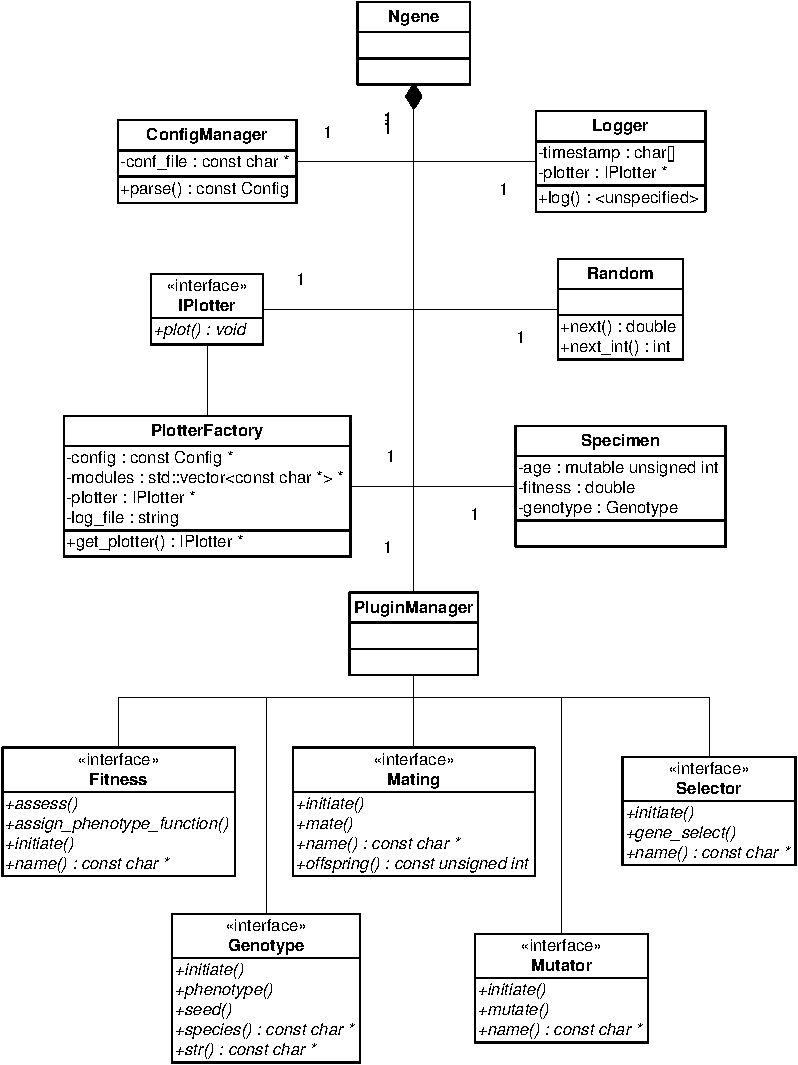
\includegraphics[scale=0.9]{diagram_ngene}
	\caption{Overview of Ngene}
	\label{fig:diagram_ngene}
\end{figure}

Figure~\ref{fig:diagram_ngene} shows a brief overview of how Ngene is put together.

When the program starts up, Ngene will start parsing a configuration file. It finds this file either via the path passed as parameter on execution, or it will simply start looking for the default one. The module responsible for this, \texttt{ConfigManager}, will create a structure storing the configuration and pass it to \texttt{PluginManager}.

\texttt{PluginManager} handles all loading and unloading of modules specified in a configuration file. If all modules load successfully, it also acts as an interface through which the core communicates with the modules. \texttt{PluginManager} will automatically unload modules and release all resources when the program exits.

Ngene talks with its modules via predefined interfaces, as can be seen directly under \texttt{PluginManager} in figure~\ref{fig:diagram_ngene}. All methods in these modules must be implemented in order to be compatible with Ngene. A more detailed description of what these methods do and sample code can be found in the system documentation. Besides these restrictions, a user can extend the system in any way they see fit.

All logging of runs are done in \texttt{Logger}. On first call, it will make sure that the user has writing privileges and, on successive calls, plot a graph of the progression. When the program terminates, it will also create a file output of the best specimen - the format of which is specified in the \texttt{Genotype} module. The format can be anything from a simple text file to a proprietary format specified by the user.

The genetic algorithm starts by populating the adult population, a responsibility of the \texttt{Genotype} module. The randomly generated genotypes are stored in \texttt{Specimen}s in an array, or vector, that will make up the adult population. When this vector is full (a configurable value), the genetic algorithm will run for a given number of generations (also configurable) or until a perfect \texttt{Specimen} is found, i.e. \texttt{fitness = 1.0}.


\subsection{Ngene Development Framework}
\begin{figure}[!ht]
	\centering
	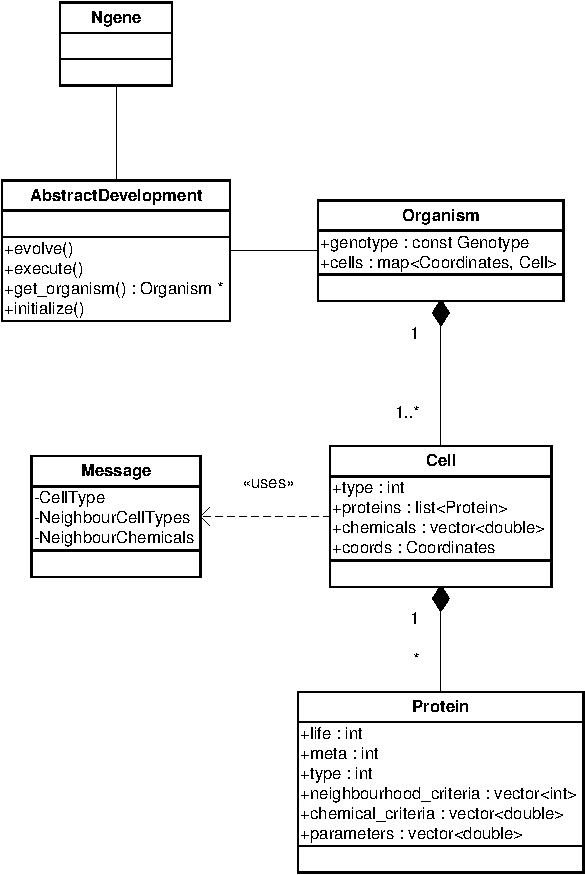
\includegraphics[scale=0.9]{diagram_ndevframe}
	\caption{Overview of Ngene Development Framework}
	\label{fig:diagram_ndevframe}
\end{figure}

To further extend the genetic algorithm already implemented in Ngene, a generic development framework will provide an easier way to test computational development models. The framework is designed to accommodate any conceivable model.

It consists of a common code base that implements common algorithms and concepts such as a cell or a protein (see fig.~\ref{fig:diagram_ndevframe}) and is enforced in order to ensure a common ground on which a comparison between different development models can be done while minimizing any implementation factors that may give one model an advantage over the other. In other words, it will take care of notifying all cells of a development step, or a tick, and all inter-cellular communications (see fig.~\ref{fig:diagram_ndevframe_msg}).

\begin{figure}[!ht]
	\centering
	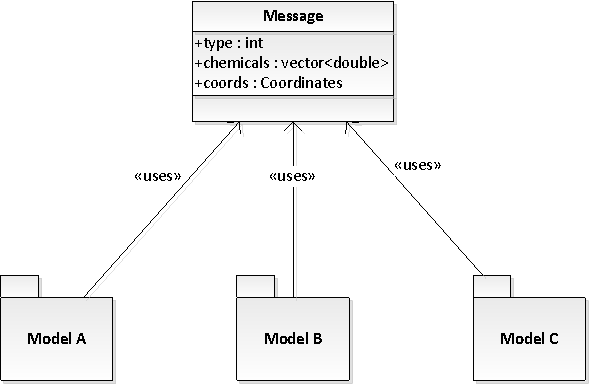
\includegraphics[scale=0.9]{diagram_ndevframe_msg}
	\caption{A common message implementation should eliminate factors involving what information is exchanged between the organism's cells.}
	\label{fig:diagram_ndevframe_msg}
\end{figure}

Figure~\ref{fig:diagram_ndevframe_common-base} shows three different scenarios where model A and B use only chemicals, while model C only makes use of proteins. This tells us that model A and B may use both the cell type and the chemicals part of a \texttt{Message}, while model C only takes cell type into consideration (or it may not even implement cell communication). We also see that model B and C make use of a control program besides the genome. Even though these three models are different, they still use the same framework, meaning all underlying code is the same. A comparison can then be done without fearing that there are implementation differences that may affect one model or another.

\begin{figure}[!ht]
	\centering
	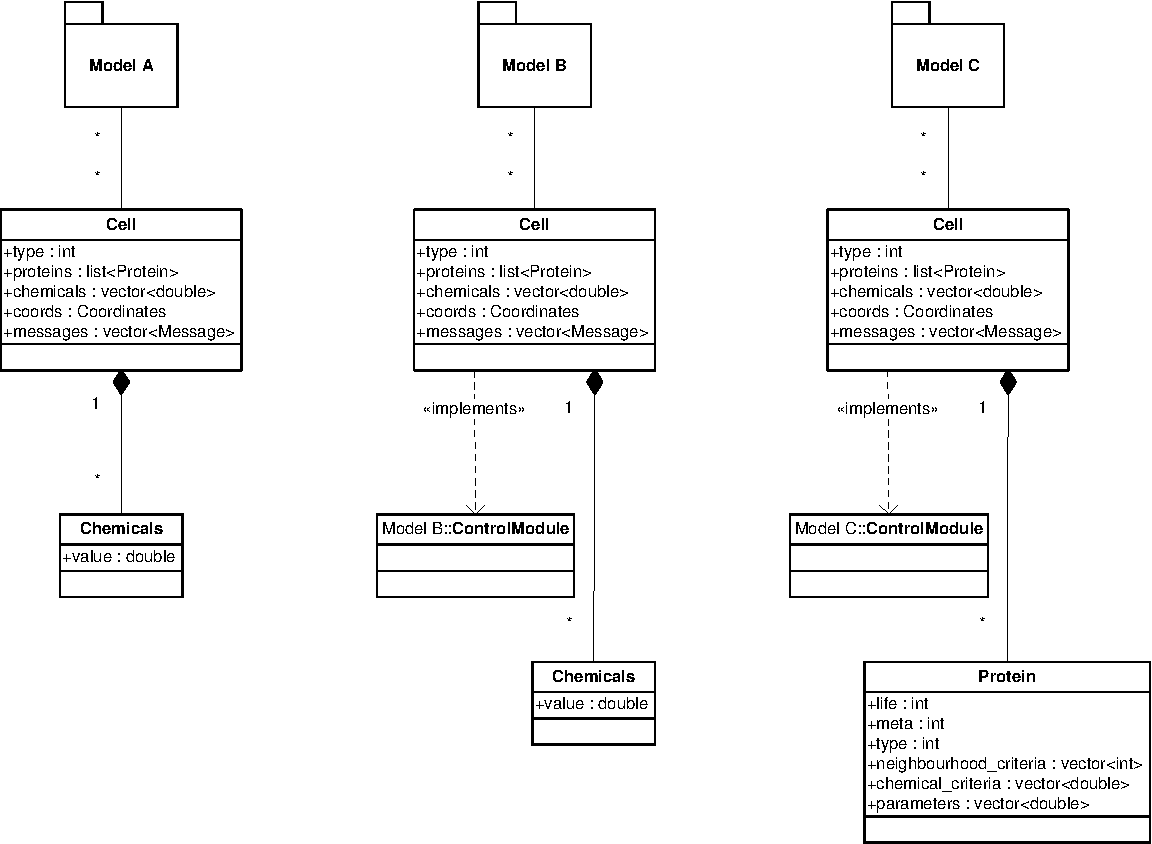
\includegraphics[scale=0.8]{diagram_ndevframe_common-base}
	\caption{Albeit different, all three models still use the same implementation of a cell, chemicals and proteins, and receive the same messages.}
	\label{fig:diagram_ndevframe_common-base}
\end{figure}


\subsubsection{Using the Framework}
\begin{figure}[!ht]
	\centering
	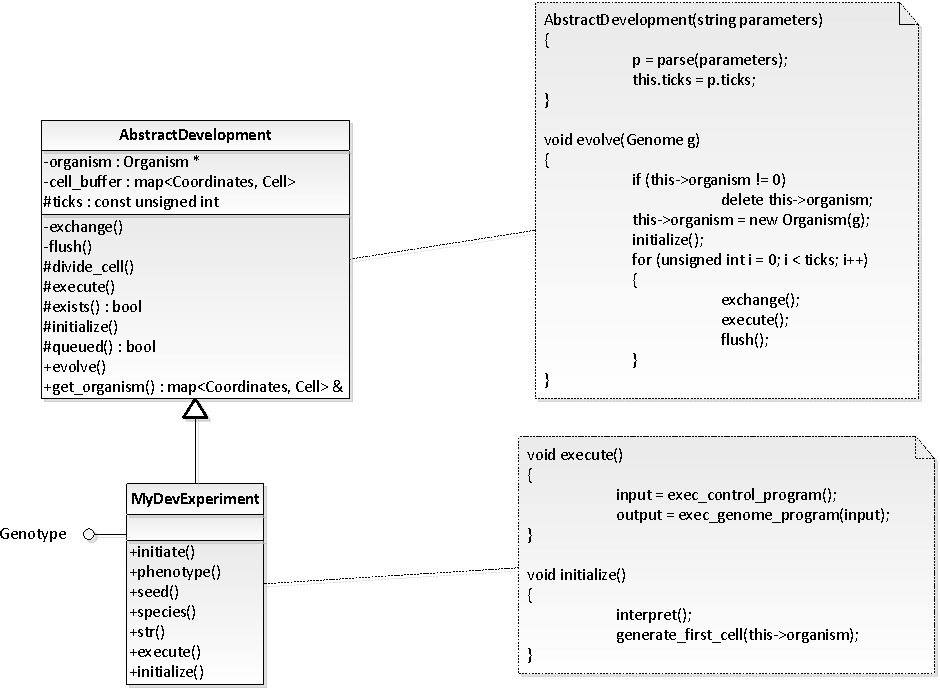
\includegraphics[scale=0.9]{diagram_ndevframe_ex}
	\caption{An example of how one can implement \texttt{MyDevExperiment}.}
	\label{fig:diagram_ndevframe_ex}
\end{figure}

A module is created by inheriting \texttt{AbstractDevelopment} (see fig.~\ref{fig:diagram_ndevframe_ex}) and implementing the required methods, \texttt{execute()} and \texttt{initialize()}. The latter is executed every time a new organism is to be developed and can be used to expand the genotype into a more functional object, such as an actual cell program, and preparing the organism with initial cells. The \texttt{execute()} method is called every tick, for every cell in the organism. Here, the cell program from the genotype can be executed as well as any control programs that might be needed. Note that any messages sent has already been received and are stored in the cells themselves by the time the first cell is given the chance to fulfil its purpose in a tick. It will not be possible to actually access the organism itself in this method to avoid tampering with and further minimize any differences between two models.

With regards to speed optimizations, lots of thought as been put into how to represent the organisms themselves. In the current implementation, an \emph{STL Map} is used to store the cells using their coordinates as the key value. Other alternatives were also considered:

\begin{center}
	\begin{tabular}{ r | c | c | c }
		~ & STL \texttt{<map>} & STL \texttt{<vector>} & STL \texttt{<ext/hash\_map>} \\
		\hline
		element access & $O(log~n)$ & $O(1)$ & $O(1)$ \\
		\hline
		insertion & $O(log~n)$ & $O(1)$ & $O(1)$ \\
		\hline
		search & $O(log~n)$ & $O(n)$ & $O(1)$ \\
	\end{tabular}
\end{center}

A quick glance at the comparison table and the \texttt{<ext/hash\_map>} may seem like the best choice to go with. However, there are some drawbacks that must be taken into consideration. A good hashing algorithm is essential for the performance of the hash table by providing a uniform distribution over the array. Too simple, and a lot of collisions will occur, but too complex and the hashing table will spend all of its time calculating a hash value. Collisions will, however, occur regardless of how good the algorithm is. The \emph{birthday paradox} predicts that it doesn't take many elements before the chance of a collision exceeds 95\%, even for very big arrays. A good collision resolution is therefore also needed but it will not be enough to guarantee the performance advantage over other solutions. For the experiments conducted in this thesis, the number of cells rarely exceeded 1000. For a \texttt{<map>}, this means at most 10 comparisons to find an element by its key value. A hash table would require about the same number of operations to calculate the hash, perform the lookup and resolve any collisions.

The \texttt{<map>} was chosen over the \texttt{<vector>} because despite its better access and insertion times, required more time to find all of a cell's neighbours. This could've be remedied by creating and maintaining a neighbours list for every cell. However, this would make insertion $O(n)$ as opposed to $O(log~n)$ of the \texttt{<map>}.


\subsubsection{ArtDev3D}
A simpler (and hopefully faster) version of Johan H{\o}ye's master's thesis\cite{hoye2006} model was implemented within the framework. Though simpler, all logical operations are still kept intact.

Due to lack of proper system documentation, porting the code from Java to C++ has been a rather cumbersome job. Many biology concepts made their way into his code, making it very messy and difficult to read at times. There are classes for pretty much every concept such as \texttt{Cell}, \texttt{Protein} and even \texttt{Proteincollection} and \texttt{ChangeChemicalConcentrationInCellProtein}. Because of how the hierarchy is built up, functions may call other functions which again call different functions, and so on, to perform simple operations. These functions are often called many times in a single cell during a single tick, putting a strain on the call stack when there are a lot more cells in an organism, more ticks in a development process, and many organism in a population that are to evolve over generations. Parts of the effort in porting this model over to the new framework has been spent on flattening the structure a bit, hopefully making it simpler and easier to understand. In many cases, it was simply substituting a class, such as \texttt{Chemicalconcentrations}, with an STL container. After all, the golden rule of programming is to not write custom containers unless deemed absolutely necessary.

There are a couple of issues that Johan may have missed when he wrote his thesis. A lot of papers in this field agree to a certain degree that cells develop simultaneously, i.e. for all development that is based on neighbouring cells' states, an information exchange between all cells should occur first, and any other cellular operations last. However, in Johan's model, this is not implemented. The following snippets from his code should demonstrate this issue.

\begin{verbatimtab}
development/model/DevelopmentProsess.java:287-307:

/*
 * Performs a tick.
 * The development prosess steps one step forwards.
 */
private boolean doTick() {
	int cTime = getCurrentTick();
	int dTime = this.numberOfTicks;
	boolean success = false;

	if(cTime < dTime) {
		[...]
		this.currentOrganism.tickEvent(); //< Development occurs here
		this.currentTick++;
		success = true;
	} else {
		setActive(false);
	}
	return success;
}
\end{verbatimtab}

A tick signalizes the organism to start doing something. Here, a tick event is triggered in an organism a certain amount of times.

\begin{verbatimtab}
development/model/framework/organism/Organism.java:90-101:

/**
 * Informs all cells in this organism of a tick event.
 * Each time this method is called, the development proceeds one step.
 * This method should be called each time a tick happens in
 * {@link DevelopmentProsess}
 */
public void tickEvent() {
	[...]
	// notify each cell of the tick
	for (Cell c : cells) {
		c.tickEvent();
	}
}
\end{verbatimtab}

The organism receives the event and then relays this tick event to all cells inside of it. This occurs in the order in which the cells were added to the array.

\begin{verbatimtab}
development/model/framework/cell/Cell.java:275-293:

/**
 * Handles the actions this cell must do each tick.
 * The order in which the different processes are carried out may have a great
 * effect on the behaviour of the cell. Great care must be taken if changing
 * this method!
 *
 */
public final void tickEvent() {
	[...]

	// Clears all requested actions
	resetRequestedActions();

	// This cells protein collection is doing their action
	pc.tickEvent();

	// This cell is doing its action
	doAction();
}
\end{verbatimtab}

Here we see that all requested actions by this cell's proteins are deleted before new actions can be requested. This happens in \texttt{pc.tickEvent()}: First, all dead proteins are removed from the collection and the remaining are aged. Finally, these proteins can request an action upon the cell based on chemical levels in the cell, as well as criteria based on neighbouring cells' types. These queued actions are accumulated and realized in \texttt{doAction()}.

We see that \texttt{Cell.tickEvent()} performs both the information gathering and all the actions as a single function while they should have been split up and run in two different loops. The problem here is that a single cell may get ``newer'' information from a neighbouring cell that already has been processed mixed up with ``older'' information from unprocessed cells, what it should have based its actions on.

For the purpose of my thesis, \texttt{doAction()} has been extracted out of \texttt{Cell.tickEvent()} and is called separately in another loop. This may or may not have a consequence in the outcome of the runs. The experiments conducted will show whether or not this is the case.


\subsubsection{Julian F. Miller's Model}
This model is based a number of works such as \cite{mteurogp2000} and \cite{ecal2003}. There are no official documentation or source code of it, so all work is based solely on descriptions of how it works.
